\chapter{Logical dependencies in key class detection}
\label{cap:key_class_detection}

\section{Introduction and research questions}
\label{sec:key_introduction}
\hspace{4em}Zaidman et al. \cite{ZaidmanJurnal} were the first to introduce the concept of \emph{key classes}, referring to classes found in documents written to provide an architectural overview of the system or an introduction to the system structure.

Key class identification has been previously done using structural dependencies \cite{PagerankENASE}, \cite{enase15}, \cite{PagerankSACI}. In this chapter, key classes are identified using dependencies extracted from the version control system combined with dependencies from the source code. The analysis is performed both separately and together to see how the final results fluctuate depending on the type of dependency used.

The analysis in this chapter is performed on three open-source projects: Ant, Tomcat Catalina, and Hibernate. For this chapter, the following research questions are addressed:

\emph{RQ1: Can combining logical and structural dependencies improve the previous results obtained by using only structural dependencies in key class detection?}  
Since logical dependencies overlap only in a small percentage with structural dependencies, the goal is to combine both dependencies and provide them as input to key class identification tools.

\emph{RQ2: Can logical dependencies alone provide good results in key class detection?}  
This question focuses on using logical dependencies as stand-alone inputs. Although logical dependencies are different than structural dependencies, they may still provide enough system information to be successfully used as input for tools like key classes detection tools.

\emph{RQ3: Does applying the connection strength filter have a positive impact on key class detection?}  
The connection strength filter and the commit size filter will be used to filter co-changes into logical dependencies. The goal is to evaluate whether this new strength filter outperforms the confidence and support filter in key class detection \cite{b4}.






\section{Related work on key class detection} %not refactored
\label{sec:key_related_work}

\hspace{4em}Zaidman et al. \cite{ZaidmanJurnal} were the first to introduce the concept of key classes, referring to classes commonly found in documents that provide an architectural overview of the system or an introduction to its structure. 

Tahvildari and Kontogiannis offered a more detailed definition of key classes: “Usually, the most important concepts of a system are implemented by very few key classes which can be characterized by specific properties. These classes, which we refer to as key classes, manage many other classes or use them in order to implement their functionality. The key classes are tightly coupled with other parts of the system. Additionally, they tend to be rather complex since they implement much of the legacy system’s functionality” \cite{Tahvildari2004ImprovingDQ}.

Other researchers have used similar concepts under different terms, such as important classes \cite{Meyer2014IdentifyingIC} or central software classes \cite{CentralClassesSteidl}. 

Key class identification can be performed using different algorithms and input types. In the research by Osman et al., key class identification is performed using a machine learning algorithm with class diagrams as input \cite{6676885}. Thung et al. build on Osman et al.’s approach by incorporating network metrics and optimistic classification to enhance key class detection \cite{rocclasification}. 

Zaidman et al. \cite{ZaidmanJurnal} apply a web-mining algorithm and dynamic source code analysis to identify key classes. Similarly, Sora et al. use a PageRank-inspired algorithm combined with static source code analysis \cite{PagerankENASE}, \cite{enase15}, \cite{PagerankSACI}. In \cite{Finding-key-classes}, the authors extend this approach by including additional class attributes to improve key class identification. 

The PageRank algorithm, developed initially for ranking web pages \cite{ilprints422}, works based on a recommendation system. If one node is connected to another, it recommends the second node. In previous studies, connections were based on structural dependencies extracted from static code analysis. If class A has a structural dependency with class B, both A and B recommend each other.

Based on their importance, the ranking algorithm assigns a score to all classes from the analyzed system's source code. To distinguish important classes from the rest, a threshold for the TOP-ranked classes is set. The TOP threshold value can range from 1 to the total number of classes in the system. 

Some researchers \cite{ZaidmanJurnal}, \cite{Ding2016AnIA}, \cite{PAN2018188} suggest that 15\% of the total number of classes in the system is a suitable value for the TOP threshold. Others \cite{Finding-key-classes} argue that 15\% is too high and propose a range of 20 to 30 classes as a more appropriate threshold \cite{b4}.

\section{Methodology and implementation}
\label{sec:key_methodology_implementation}

\hspace{4em}This section presents the methodology and implementation used for key class detection. Section \ref{subsec:key_evalmetrics} describes the evaluation metrics used to assess the results of detected key classes. Section \ref{subsec:key_previous_measurements} describes the baseline approach by Şora et al. \cite{Finding-key-classes}. Section \ref{subsec:key_current_approach} describes the current approach, which extends the baseline by incorporating logical dependencies from the version control system. Section \ref{subsec:key_tool} describes the tool setup and workflow used for extracting, filtering, and processing logical dependencies and using them for key class detection.


\subsection{Metrics for results evaluation} %not refactored
\label{subsec:key_evalmetrics}

\hspace{4em}To evaluate the quality of the key classes ranking algorithm and solution produced, the key classes found are compared with a reference solution.

The reference solution is extracted from the developer documentation. Classes mentioned in the documentation are considered key classes and form the reference solution (ground truth) used for validation \cite{7551990}. A classification model is then used to compare the two solutions. The quality of the solution produced is evaluated by using metrics that evaluate the performance of the classification model, such as Precision-Recall and Receiver Operating Characteristic Area Under Curve (ROC-AUC). 

A classification model (or "classifier") is a mapping between expected results and predicted results \cite{ROCIntro}, \cite{ROCBRADLEY19971145}. Both results can be labeled as positive or negative, which leads us to the confusion matrix from figure \ref{fig:confusion} \cite{b4}. 
\begin{figure}[h]
\centering
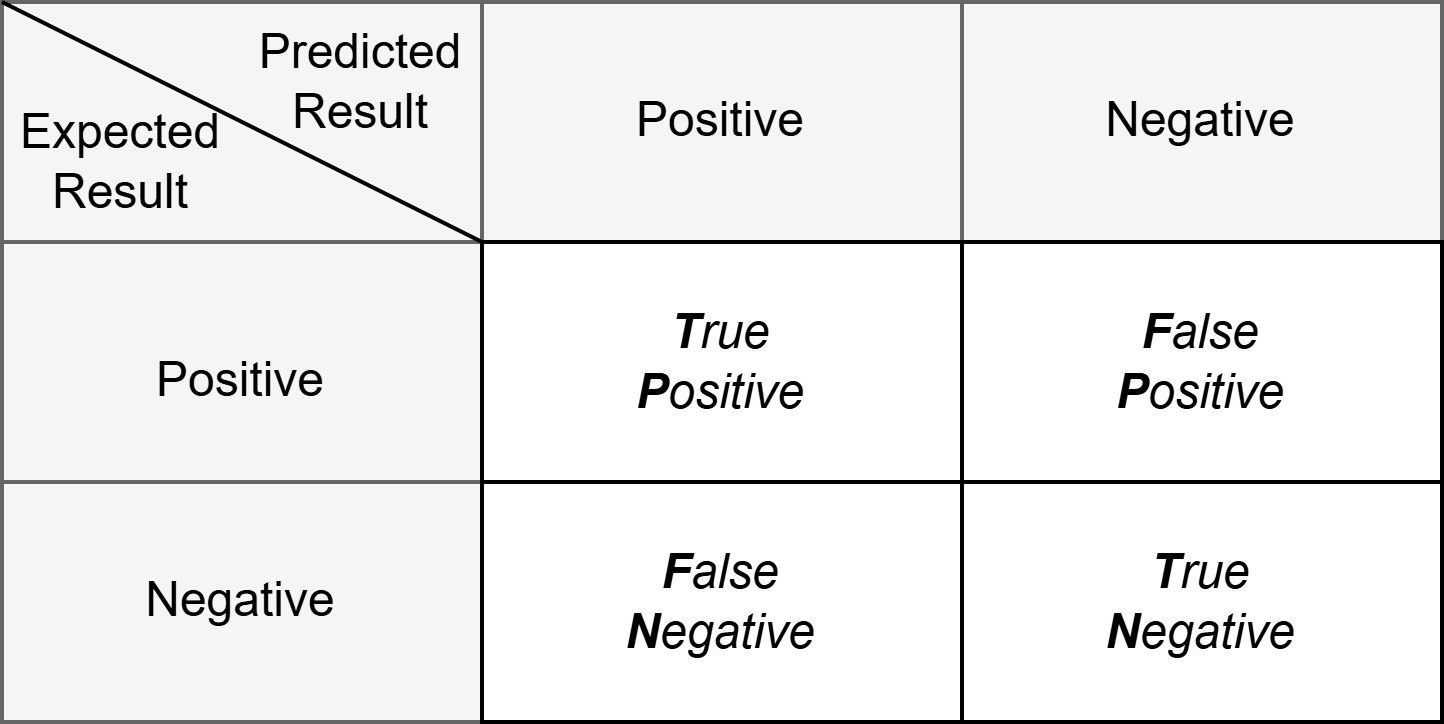
\includegraphics[scale=0.9]{confusion.png}
\caption{Confusion matrix}
\label{fig:confusion}
\centering
\end{figure}
The confusion matrix has the following outcomes:\\
- \textit{true positive}, if the expected result is positive and the predicted result is also positive.\\
- \textit{false positive}, if the expected result is positive but the predicted result is negative.\\
- \textit{false negative}, if the expected result is negative but the predicted result is positive.\\
- \textit{true negative}, if the expected result is negative and the predicted result is also negative.



\underline{\textit{Precision-recall}}


\hspace{-4em}Precision is the ratio of True Positives to all the positives of the result set.

\begin{equation}
 precision = \frac{TP}{TP+FN}
\end{equation}
The recall is the ratio of True Positives to all the positives of the reference set.

\begin{equation}
 recall = \frac{TP}{TP+FP}
\end{equation}

To distinguish the key classes from the rest of the classes a TOP threshold is used. Some researchers consider that 15\% of the total classes is the best value for the TOP threshold and others consider that the value should be in the range of 20-30. 

The precision-recall metric is suited if the threshold value is fixed. If the threshold value is variable, then metrics that capture the behavior over all possible values must be used. Such metric is the Receiver Operating Characteristic metric.

\underline{\textit{Receiver Operating Characteristic Area Under Curve}}


The ROC graph is a two-dimensional graph that has on the X-axis plotted the false positive rate and on the Y-axis the true positive rate. By plotting the true positive rate and the false positive rate at thresholds that vary between a minimum and a maximum possible value we obtain the ROC curve. The area under the ROC curve is called Area Under the Curve (AUC).

The true positive rate (TPR) of a classifier is calculated as the division between the number of true positive results identified and all the positive results identified:

\begin{equation}
TPR = \frac{TP}{TP+FN}
\end{equation}
The false positive rate (FPR) of a classifier is calculated as the division between the number of false positive results identified and all the negative results identified:

\begin{equation}
FPR = \frac{FP}{FP+TN}
\end{equation}


The True Positives (TP) are the classes found in the reference solution and in the top TOP ranked classes. False Positives (FP) are the classes not found in the reference solution but in the TOP ranked classes.
True Negatives (TN) are classes found neither in the reference solution nor in the TOP ranked classes. False Negatives (FN) are classes found in the reference solution but not in the TOP ranked classes.

In related research, the ROC-AUC metric has been used to evaluate the results for finding key classes of software systems. For a classifier to be considered good, its ROC-AUC metric value should be as close to 1 as possible.
When the value is 1, then the classifier is considered to be perfect. A metric value between 0.8 and 0.9 means that the classifier is excellent. Between 0.8 and 0.7 means acceptable results, and between 0.7 and 0.5 means poor results \cite{ROC_METRIC_VALS, b4}. 



\subsection{Baseline approach}
\label{subsec:key_previous_measurements}

\hspace{4em}We use the research of I. Şora et al. \cite{Finding-key-classes} as a baseline for our research involving the usage of logical dependencies to find key classes. The entire workflow of the baseline approach is also presented in figure \ref{fig:baseline_approach}.

\begin{figure}[H]
\centering
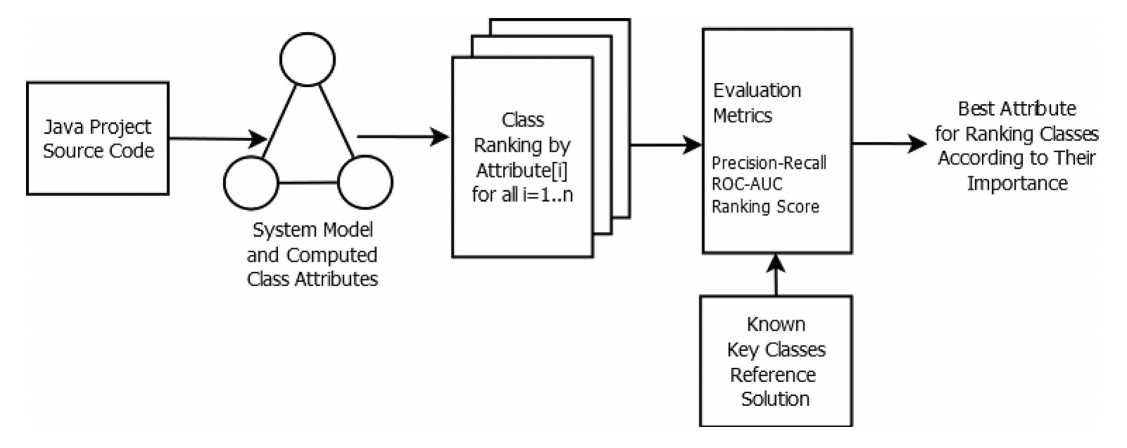
\includegraphics[width=\textwidth]{baseline_approach.PNG}
\caption{Overview of the baseline approach. Reprinted from “Finding key classes in object-oriented
software systems by techniques based on static analysis.” by Ioana Sora and Ciprian-Bogdan Chirila, 2019, Information and Software Technology, 116:106176. Reprinted with permission. }
\label{fig:baseline_approach}
\centering
\end{figure}


Şora et al. used static source code analysis, a page ranking algorithm, and additional class attributes to identify key classes \cite{PagerankENASE, enase15, PagerankSACI, Finding-key-classes}. The page ranking algorithm is a customized version of PageRank, originally developed for ranking web pages \cite{ilprints422}. It operates based on a recommendation system: if one node is connected to another, it recommends the second node. In this context, connections are established through structural dependencies. For example, if class A has a structural dependency with class B, both A and B recommend each other.

The ranking algorithm evaluates all classes from the system’s source code based on their importance. To identify the key classes from the rest, a threshold is set for the highest-ranked classes. This threshold, referred to as the TOP threshold, can range from 1 to the total number of classes in the system \cite{b4}. In the baseline approach, the TOP threshold is typically set between 20 and 30 classes.


The baseline approach involves a tool that processes the system’s source code to identify key classes and compares the results with a reference solution extracted from the developer documentation using a classification model. To rank classes by importance, various class metrics are considered \cite{Ding2016AnIA, ZaidmanJurnal, PAN2018188}. Below are some key class metrics used in the baseline approach for ranking.

\textbf{Class attributes that characterize key classes}


The metrics used in the baseline research can be grouped into the following categories: 

\begin{itemize}
	\item class size metrics: number of fields (NoF),  number of methods (NoM), global size (Size = NoF+NoM).
	\item class connection metrics, any structural dependency between two classes:
		\begin{itemize}
			\item CONN-IN, the number of distinct classes that use a class;
			\item CONN-OUT, the total number of distinct classes that are used by a class;
			\item CONN-TOTAL, the total number of distinct classes that a class uses or are used by a class (CONN-IN + CONN-OUT).
			\item CONN-IN-W, the total weight of distinct classes that use a class. 
			\item CONN-OUT-W, the total weight of distinct classes that are used by a class. 
			\item CONN-TOTAL-W, the total weight of all connections of the class (CONN-IN-W + CONN-OUT-W) \cite{Finding-key-classes}.
		\end{itemize}
	\item class pagerank values, previous research use pagerank values computed on both directed and undirected, weighted and unweighted graphs:
		\begin{itemize}
			\item PR - value computed on the directed and unweighted graph;
			\item PR-W - value computed on the directed and weighted graph;
			\item PR-U - value computed on the undirected and unweighted graph;
			\item PR-U-W - value computed on the undirected and weighted graph;
			\item PR-U2-W - value computed on the weighted graph with back-recommendations \cite{PagerankENASE}, \cite{enase15}, \cite{Finding-key-classes}, \cite{PagerankSACI}.
		\end{itemize}
\end{itemize}


Due to the fact that the TOP threshold is varied, the Receiver Operating Characteristic Area Under Curve metric is used for the evaluation of the results.



\subsection{Current approach}
\label{subsec:key_current_approach}

\hspace{4em}The baseline approach uses a tool that takes as an input the source code of the system and applies ranking strategies to rank the classes according to their importance. We modified the tool used by the baseline approach to take also the logical dependencies as input; the rest of the workflow is the same as in the baseline approach (figure \ref{fig:baseline_approach}).
\begin{figure}[H]
\centering
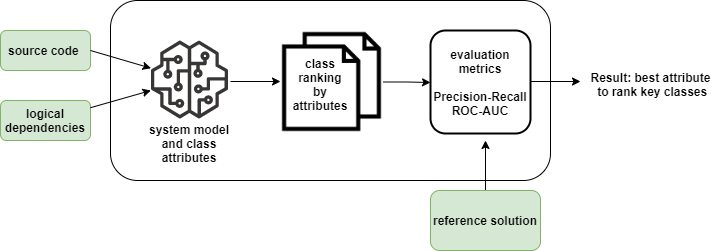
\includegraphics[scale=0.43]{current_approach.PNG}
\caption{Overview of the current approach.}
\label{fig:baseline_approach}
\end{figure}

Below are some of the class metrics used in the baseline approach and in our current research to rank the classes according to their importance. The class metrics used can be separated into two categories: class connection metrics and class PageRank values. The class connection metrics are CONN-TOTAL-W, which is the total weight of all connections of the class, and CONN-TOTAL, the total number of distinct classes that a class uses or is using the class \cite{Finding-key-classes}.

Previous research used PageRank values computed on both directed and undirected, weighted and unweighted graphs. In the current research, we use the PR, which is the PageRank value computed on the directed and unweighted graph, the PR-U, which is the value computed on the undirected and unweighted graph, and the PR-U2-W, the value computed on the weighted graph with back-recommendations \cite{PagerankENASE}, \cite{enase15}, \cite{Finding-key-classes}, \cite{PagerankSACI}.

The comparison between the current proposed approach and the baseline method is illustrated in Figure \ref{fig:baseline_comparison}. 
\begin{figure}[H]
\centering
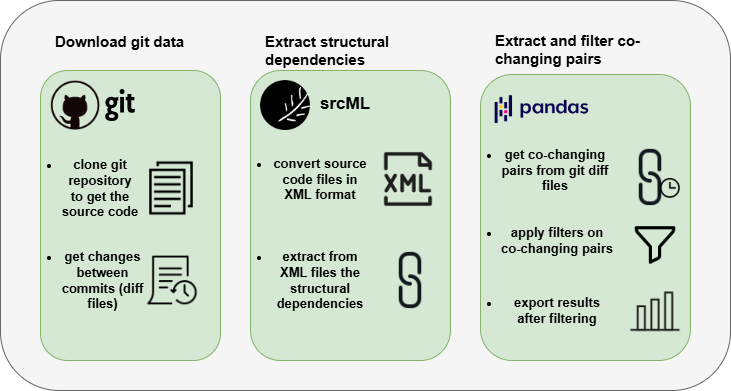
\includegraphics[width=\textwidth]{baseline_comparison.png}
\caption{ Comparison between the new approach and the baseline }
\label{fig:baseline_comparison}
\centering
\end{figure}


\subsection{Tool setup and current workflow used}
\label{subsec:key_tool}

\hspace{4em}The entire process of extracting co-changing pairs from the versioning system, filtering them, and exporting the remaining pairs is performed using the same Python tool described and used in Chapters \ref{extraction} and \ref{chap:combining_dependencies}. The entire tool workflow is presented in Figure \ref{fig:workflow_key}.

\begin{figure}[H]
\centering
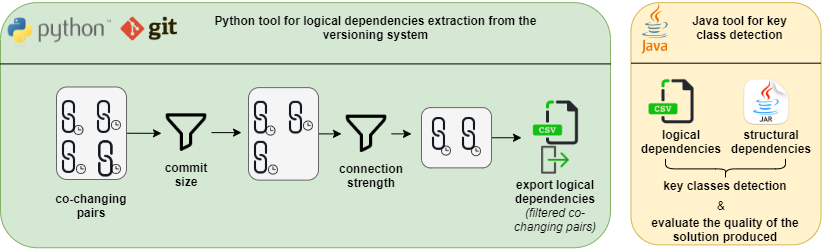
\includegraphics[width=\textwidth]{key_class_workflow.png}
\caption{Workflow for key classes detection}
\label{fig:workflow_key}
\centering
\end{figure}`


The filtering process involves applying two filters: the commit size filter and the connection strength filter. The commit size filter excludes all commits with more than 10 files \(cs \leq 10\). The connection strength filter ranges from \( \geq 10\% \) to \( \geq 100\% \), with a step of 10, resulting in 10 different sets of logical dependencies, each corresponding to a specific strength threshold. A fixed threshold is not used because the goal is to assess how strength thresholds impact key class detection results. After filtering, the remaining co-changing pairs are exported to CSV files.

The next step is to use the exported logical dependencies for key class detection. The same key class detection tool described in Section \ref{subsec:key_previous_measurements} is used, with adaptations to support logical dependencies. Previously, the tool processed only structural dependencies extracted from the system's source code. The tool ranks the top key classes and evaluates the results using the ROC-AUC metric.





\section{Data set used in experimental analysis}
\label{sec:key_dataset}


\hspace{4em}The research of I. Şora et al. \cite{Finding-key-classes}, which we use as our baseline, was conducted on the object-oriented systems listed in Table \ref{tab:keyclass:overview} \cite{b4}. For a system to be suitable for investigation using logical dependencies, it needs to meet several criteria: it must be hosted on GitHub/Bitbucket, have release tags to identify specific versions, and contain a considerable number of commits. Out of the 14 object-oriented systems mentioned in the paper \cite{Finding-key-classes}, 13 have corresponding GitHub repositories, as shown in Table \ref{tab:gitfoundsystems}. From these, only six repositories have release tags matching the versions specified in Table \ref{tab:keyclass:overview}. Finding the correct release tags is important to filter commits by date, ensuring that only commits made before the specified release are considered.

The number of commits found in these six repositories ranges from 19,108 for Tomcat Catalina to 149 for JHotDraw. Since a significant number of commits is important for obtaining accurate results, we concluded that only three systems could be used for key class detection using logical dependencies: Apache Ant, Hibernate, and Tomcat Catalina. Among these, Apache Ant is the most frequently analyzed system in other studies \cite{enase19}, \cite{7332515}, \cite{1402122}, \cite{Kamran2016IdentificationOC}.

\begin{table}[H]
\renewcommand{\arraystretch}{1.8}
\caption{Analyzed Software Systems in Previous Research.}
\label{tab:keyclass:overview}
\centering
\resizebox{\textwidth}{!}{
\begin{tabular}{|c|l|p{9cm}|c|}
\hline
\textbf{ID} & \textbf{System} & \textbf{Description} & \textbf{Version} \\
\hline
S1 & Apache Ant & Java library and command-line tool that manages build processes through targets and extension points & 1.6.1 \\
S2 & Argo UML & UML modeling tool with support for all UML diagrams & 0.9.5 \\
S3 & GWT Portlets & Open-source web framework for building GWT (Google Web Toolkit) applications & 0.9.5 beta \\
S4 & Hibernate & Persistence framework for Java & 5.2.12 \\
S5 & javaclient & Java distributed application for interacting with robots & 2.0.0 \\
S6 & jEdit & Java-based mature text editor for programmers & 5.1.0 \\
S7 & JGAP & Genetic Algorithms and Genetic Programming Java library & 3.6.3 \\
S8 & JHotDraw & Two-dimensional graphics framework for structured drawing editors written in Java & 6.0b.1 \\
S9 & JMeter & Java application designed for load testing and performance measurement & 2.0.1 \\
S10 & Log4j & Logging service for Java applications & 2.10.0 \\
S11 & Mars & Java-based simulation project modeling human settlements on Mars & 3.06.0 \\
S12 & Maze & Maze-solver project simulating an AI algorithm navigating a maze & 1.0.0 \\
S13 & Neuroph & Java neural network framework & 2.2.0 \\
S14 & Tomcat Catalina & Open-source implementation of JavaServlet and JavaServerPages technologies & 9.0.4 \\
S15 & Wro4J & Web resource optimizer for JS and CSS in Java projects & 1.6.3 \\
\hline
\end{tabular}
}
\end{table}




\begin{table}[H]
\renewcommand{\arraystretch}{1}
\caption{Found systems and versions of the systems in GitHub. }
\label{tab:gitfoundsystems}
\centering
\scalebox{0.8}{
\begin{tabular}{|c|c|c|c|c|}
\hline
ID	&	System	&	Version	&	Release Tag name	&	Commits number	\\
\hline
\rowcolor{lightgreen}
Sl	&	Apache Ant	&	1.6.1	&	rel/1.6.1	&	6713	\\
S2	&	Argo UML	&	0.9.5	&	not found	&	0	\\
S3	&	GWT Portlets	&	0.9.5 beta	&	not found	&	0	\\
\rowcolor{lightgreen}
S4	&	Hibernate 	&	5.2.12	&	5.2.12	&	6733	\\
S5	&	javaclient	&	2.0.0	&	not found	&	0	\\
S6	&	jEdit	&	5.1.0	&	not found	&	0	\\
S7	&	JGAP	&	3.6.3	&	not found	&	0	\\
S8	&	JHotDraw	&	6.0b.1	&	not found	&	149	\\
S9	&	JMeter	&	2.0.1	&	v2\_1\_1	&	2506	\\
S10	&	Log4j	&	2.10.0	&	v1\_2\_10-recalled	&	634	\\
S11	&	Mars	&	3.06.0	&	not found	&	0	\\
S12	&	Maze	&	1.0.0	&	not found	&	0	\\
S13	&	Neuroph	&	2.2.0	&	not found	&	0	\\
\rowcolor{lightgreen}
S14	&	Tomcat Catalina	&	9.0.4	&	9.0.4	&	19108	\\
S15	&	Wro4J	&	1.6.3	&	v1.6.3	&	2871	\\
\hline
\end{tabular}
}
\end{table}

\hspace{-4em}\underline{\textbf{Version control details}}

Figures \ref{fig:strength_overview_ant}, \ref{fig:strength_overview_hibernate}, and \ref{fig:strength_overview_catalina} provide an overview of the co-change relationships within the analyzed systems. The dots represent the maximum number of updates (co-change occurrences) between two entities, while the black line shows the average occurrence value across the system.

To avoid cluttering the plots, only the maximum occurrences between entities are displayed. Even with only the maximum occurrences plotted,  most points are still located near the bottom of the graph, showing that most entity pairs have low co-change frequencies. Including all occurrences would not change the overall system view, as the additional points would only form a denser line closer to the graph’s baseline \cite{b4}.



\begin{figure}[H]
\centering
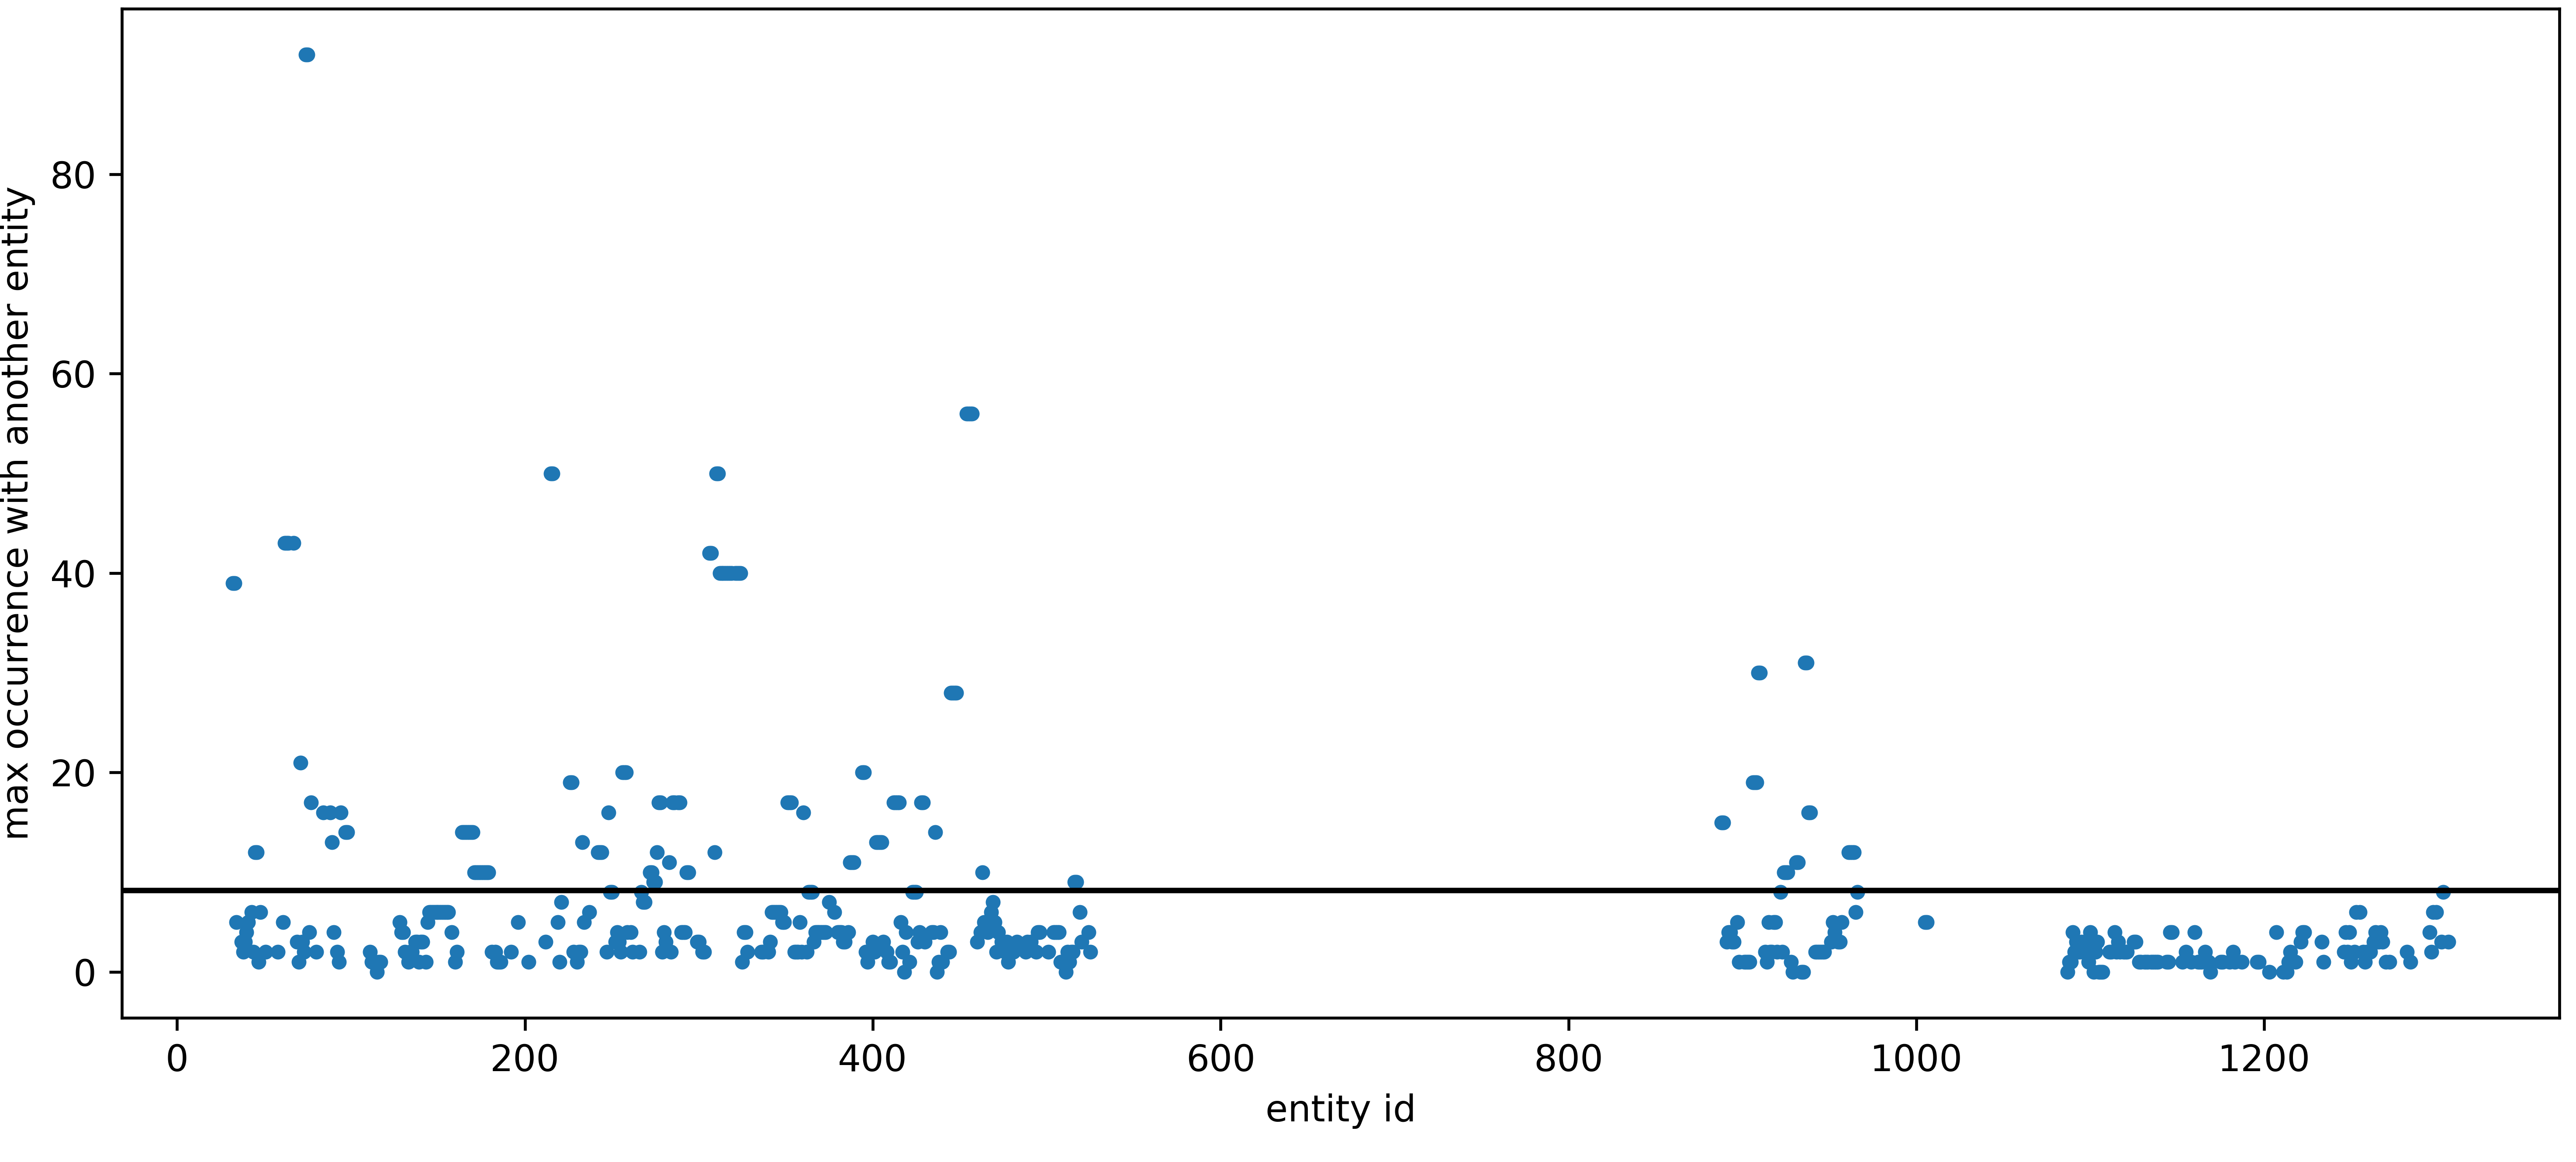
\includegraphics[width=\textwidth]{fig_ant_maxOcc.png}
\caption{Overview of the number of occurrences in Ant. }
\label{fig:strength_overview_ant}
\centering
\end{figure}

\begin{figure}[H]
\centering
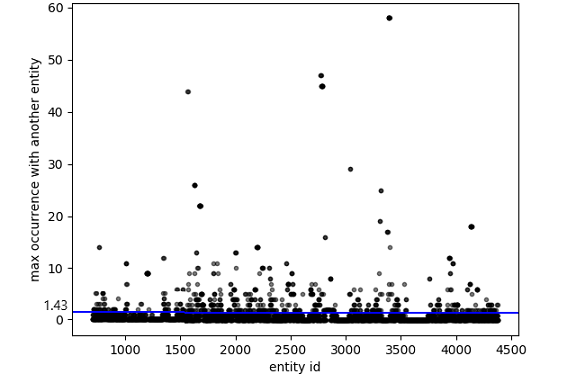
\includegraphics[width=\textwidth]{fig_hibernate_maxOcc.png}
\caption{Overview of the number of occurrences in Hibernate. }
\label{fig:strength_overview_hibernate}
\centering
\end{figure}


\begin{figure}[H]
\centering
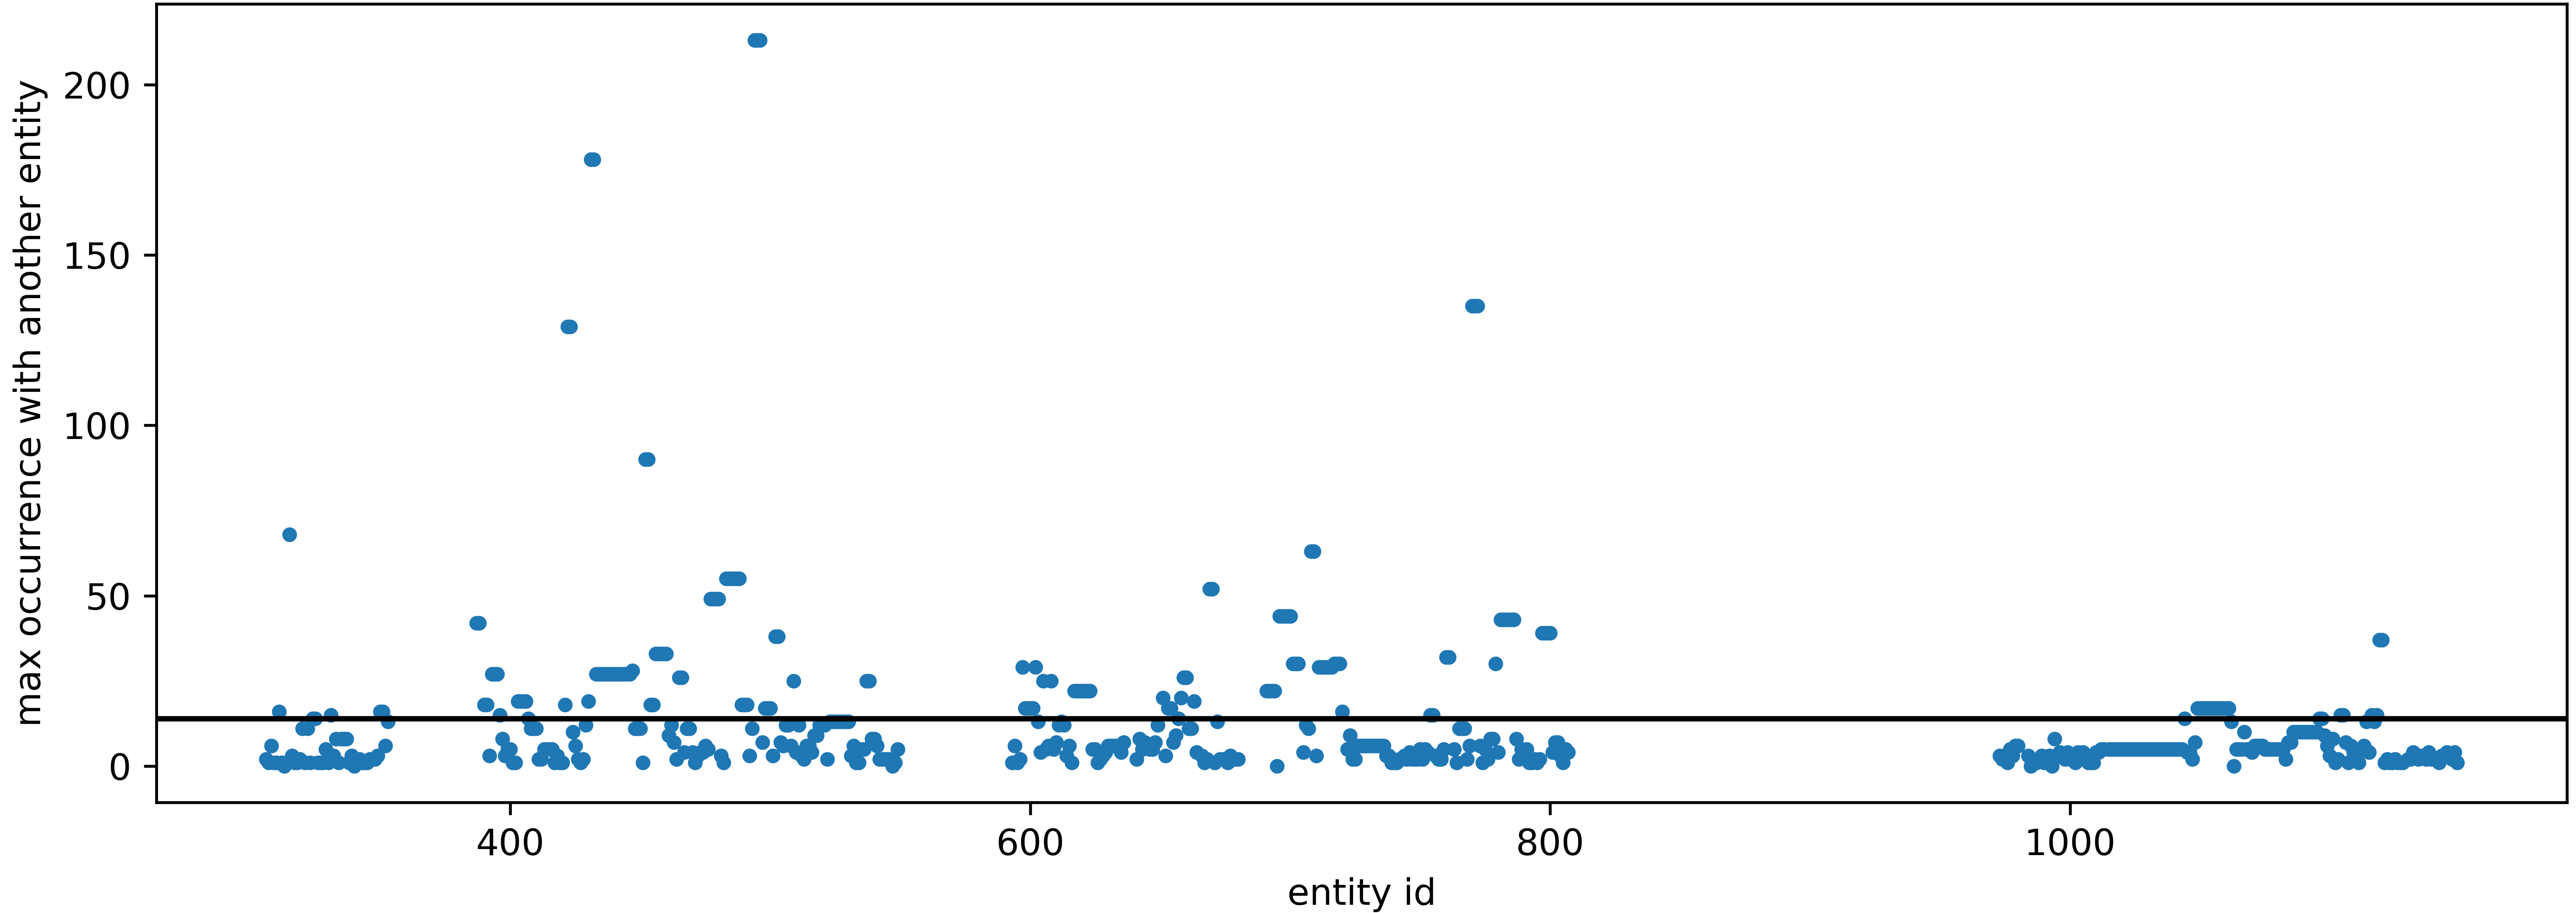
\includegraphics[width=\textwidth]{fig_catalina_maxOcc.png}
\caption{Overview of the number of occurrences in Catalina. }
\label{fig:strength_overview_catalina}
\centering
\end{figure}

To get an overview of the comparison between the number of co-changing pairs and structural dependencies at each filtering step, we plotted the data for two systems: a small-sized system (Ant) and a medium-sized system (Hibernate), as shown in Figure \ref{fig:strength_overview}. The plot includes the number of structural dependencies, co-changing pairs before filtering, and co-changing pairs after filtering. When applying the connection strength filter, the small-sized system (Ant) kept some co-changing pairs even after filtering instead of losing them all.

\begin{figure}[H]
\centering
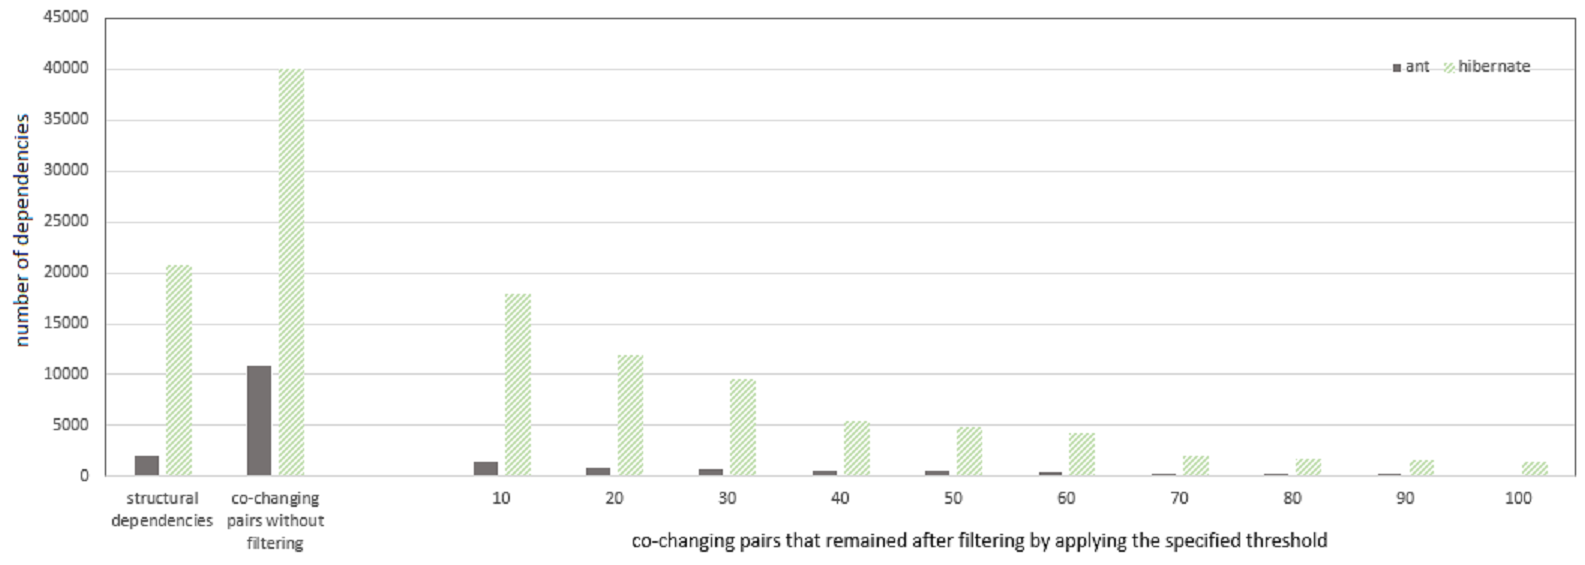
\includegraphics[width=\textwidth]{strength_overview.PNG}
\caption{Overview of the impact of connection strength filtering on the number of co-changing pairs. }
\label{fig:strength_overview}
\centering
\end{figure}

\section{Experimental plan and results}
\label{sec:key_plan_and_results}

\hspace{4em}In this section, we present our experimental plan and the results obtained. Section \ref{subsec:key_plan} describes the experimental plan that guided our research. Section \ref{subsec:key_results_baseline} describes the baseline results obtained using only structural dependencies. In Section \ref{subsec:key_results_combined}, we describe how adding logical dependencies impacts the detection process when combined with structural dependencies, while in Section \ref{subsec:key_results_ld}, we describe the results of using only logical dependencies. In Section \ref{sec:measure_metrics}, we compare the impact of using the connection strength filter versus the confidence metric filter for logical dependencies. 


\subsection{Experimental plan}
\label{subsec:key_plan}

\hspace{4em}Our research regarding logical dependencies usage in key class detection was guided based on the following research questions: \textbf{RQ1:} \textit{Can combining logical and structural dependencies improve the previous results obtained by using only structural dependencies in key class detection?} \textbf{RQ2:} \textit{Can logical dependencies alone provide good results in key class detection?} \textbf{RQ3:} \textit{Does applying the connection strength filter have a positive impact on key class detection?}

To answer the research questions, we defined the following experimental plan: 
We will use the tool mentioned in section \ref{subsec:key_current_approach}. Previously, the tool had the structural dependencies of the system and the reference solution as input, and the output was the ROC-AUC score. The closer the ROC-AUC score is to 1, the better the results. With the slightly modified version of the tool, we can give as input also logical dependencies.


For \textbf {RQ1}, we will give as input to the tool the structural and the logical dependencies, and we will compare the ROC-AUC scores obtained with the results obtained by using only structural dependencies.


\noindent\fbox{%
    \parbox{\textwidth}{%
      \textit{Hypothesis:} Key classes detection is better when we provide both types of dependencies as input to the tool. The output has a higher ROC-AUC score than the base approach.
    }%
}
\medskip

Our findings for this research question can be found in section \ref{subsec:key_results_combined}.


For \textbf {RQ2}, we will give as input to the tool only logical dependencies, and we will compare the ROC-AUC scores obtained with the results obtained by using only structural dependencies, and by using structural and logical dependencies combined.
We do not expect that the results will be better compared to the results previously obtained, but we expect results that have a ROC-AUC score close to those values. That would mean that logical dependencies can provide enough information to detect most of the key classes of the system \cite{b4}.

\medskip

\noindent\fbox{%
    \parbox{\textwidth}{%
      \textit{Hypothesis:} The output has a ROC-AUC score between 0.7 and 1. 
    }%
}

\medskip

Our findings for this research question can be found in section \ref{subsec:key_results_ld}.

For \textbf {RQ3}, we will generate two sets of logical dependencies. One set will be generated with the connection strength filter and one with the confidence filter. We will then use each set in two different scenarios: one when we only use logical dependencies to detect key classes and one when we use logical and structural dependencies for detection. Finally, we will compare the results obtained. We expect that the connection strength filter will generate better results. 

\medskip

\noindent\fbox{%
    \parbox{\textwidth}{%
      \textit{Hypothesis:} The results obtained by using the connection strength filter are better than the ones obtained with the confidence filter. 
    }%
}

\medskip
Our findings for this research question can be found in section \ref{sec:measure_metrics}.


\subsection{Results using only the baseline approach}
\label{subsec:key_results_baseline}

\hspace{4em}Table \ref{tab:previousresults} presents the ROC-AUC values for different attributes computed for the systems Ant, Tomcat Catalina, and Hibernate using the baseline approach. We will compare these values with the new ones obtained by using logical dependencies in key class detection.

\begin{table}
\renewcommand{\arraystretch}{1}
\caption{ROC-AUC metric values extracted. }
\label{tab:previousresults}
\centering
\scalebox{0.9}{
\begin{tabular}{|c|ccc|}
\hline
Metrics &	Ant	&	Tomcat Catalina	&	Hibernate	\\
\hline

PR\_U2\_W	&	0.95823	&	0.92341	&	0.95823	\\
PR	&	0.94944	&	0.92670	&	0.94944	\\
PR\_U	&	0.95060	&	0.93220	&	0.95060	\\
CONN\_TOTAL\_W	&	0.94437	&	0.92595	&	0.94437	\\
CONN\_TOTAL	&	0.94630	&	0.93903	&	0.94630	\\
\hline
\end{tabular}
}
\end{table}

\subsection{Results using combined structural and logical dependencies}
\label{subsec:key_results_combined}

\hspace{4em}The tool used in the baseline approach runs a graph-ranking algorithm on a graph containing all the structural dependencies extracted from static source code analysis. Each edge in the graph represents a dependency, while the entities forming the structural dependencies are represented as vertices.

For the measurements in this subsection, we added the logical dependencies to the graph containing all structural dependencies. Since the graph is weighted, if a structural dependency also exists as a logical dependency, the final weight of the connection becomes the sum of the weight computed for the structural dependency and the number of commits associated with the logical dependency.

In Tables \ref{tab:measurementscombined:ant}, \ref{tab:measurementscombined:tomcat}, and \ref{tab:measurementscombined:hibernate}, each row contains the computed key class metric generated using logical dependencies extracted with the connection strength threshold specified in the column headers.

We started with logical dependencies having a connection strength metric greater than 10 and increased the value by 10 in each step until reaching 100. The last column of each table contains the results obtained using only structural dependencies, as presented in Section \ref{subsec:key_results_baseline}. To answer \textit{RQ1: Can combining logical and structural dependencies improve the previous results obtained by using only structural dependencies in key class detection?}, the results obtained by combining structural and logical dependencies are close to the previously registered values. The underlined values indicate results that are better than the previously registered values. It can be observed that, for all three systems, the best values were obtained for connection strengths between 40 and 70.

\begin{table}[!h]
\setlength\tabcolsep{3.5pt}
\caption{Measurements for Ant using structural and logical dependencies combined}
\label{tab:measurementscombined:ant}
\centering
\scalebox{0.9}{
\begin{tabular}{|c|cccccccccc|c|}
\hline
Metrics &	$\geq10$	&	$\geq20$		&	$\geq30$		&	$\geq40$		&	$\geq50$		&	$\geq60$		&	$\geq70$		&	$\geq80$		&	$\geq90$		&	$\geq100$		&	Baseline \\
\hline
PR\_U2\_W	&	0.877	&	0.880	&	0.883	&	0.888	&	0.884	&	0.880	&	0.901	&	0.924	&	0.900	&	0.891	&	0.929	\\
PR	&	\underline{0.955}	&	\underline{0.932}	&	\underline{0.936}	&	\underline{0.936}	&	\underline{0.880}	&	\underline{0.884}	&	\underline{0.887}	&	\underline{0.889}	&	\underline{0.888}	&	\underline{0.890}	&	0.855	\\
PR\_U	&	0.933	&	\underline{0.937}	&	\underline{0.936}	&	\underline{0.939}	&	\underline{0.940}	&	\underline{0.939}	&	\underline{0.941}	&	\underline{0.943}	&	\underline{0.942}	&	\underline{0.940}	&	0.933	\\
CON\_T\_W	&	0.841	&	0.839	&	0.836	&	0.838	&	0.835	&	0.849	&	0.859	&	0.872	&	0.870	&	0.874	&	0.934	\\
CON\_T	&	0.920	&	0.919	&	0.921	&	0.923	&	0.923	&	0.932	&	0.934	&	0.939	&	0.937	&	0.937	&	0.942	\\
\hline
\end{tabular}
}
\end{table}

\begin{table}[!h]
\setlength\tabcolsep{3.5pt}
\caption{Measurements for Tomcat Catalina using structural and logical dependencies combined}
\label{tab:measurementscombined:tomcat}
\centering
\scalebox{0.9}{
\begin{tabular}{|c|cccccccccc|c|}
\hline
Metrics &	$\geq10$	&	$\geq20$		&	$\geq30$		&	$\geq40$		&	$\geq50$		&	$\geq60$		&	$\geq70$		&	$\geq80$		&	$\geq90$		&	$\geq100$		&	Baseline \\
\hline
PR\_U2\_W	&	0.862	&	0.883	&	0.898	&	0.901	&	0.907	&	0.909	&	0.910	&	0.916	&	0.918	&	0.918	&	0.923	\\
PR	&	0.879	&	0.885	&	0.888	&	0.882	&	0.869	&	0.869	&	0.863	&	0.863	&	0.863	&	0.863	&	0.927	\\
PR\_U	&	0.924	&	0.930	&	0.931	&	0.932	&	0.932	&	0.932	&	0.932	&	0.932	&	0.932	&	0.932	&	0.932	\\
CON\_T\_W	&	0.868	&	0.888	&	0.901	&	0.909	&	0.914	&	0.917	&	0.918	&	0.923	&	0.925	&	0.925	&	0.926	\\
CON\_T	&	0.925	&	0.934	&	0.937	&	0.938	&	0.938	&	0.938	&	0.938	&	0.938	&	0.938	&	0.938	&	0.939	\\																							
\hline
\end{tabular}
}
\end{table}

\begin{table}[!h]
\setlength\tabcolsep{3.5pt}
\caption{Measurements for Hibernate using structural and logical dependencies combined}
\label{tab:measurementscombined:hibernate}
\centering
\scalebox{0.9}{
\begin{tabular}{|c|cccccccccc|c|}
\hline
Metrics &	$\geq10$	&	$\geq20$		&	$\geq30$		&	$\geq40$		&	$\geq50$		&	$\geq60$		&	$\geq70$		&	$\geq80$		&	$\geq90$		&	$\geq100$		&	Baseline \\
\hline
PR\_U2\_W	&	0.903	&	0.909	&	0.916	&	0.928	&	0.930	&	0.932	&	0.946	&	0.947	&	0.947	&	0.949	&	0.958	\\
PR	&	0.956	&	0.959	&	0.961	&	0.962	&	0.962	&	0.962	&	0.953	&	0.953	&	0.953	&	0.954	&	0.949	\\
PR\_U	&	0.937	&	0.941	&	0.943	&	0.947	&	0.948	&	0.948	&	0.950	&	0.950	&	0.950	&	0.950	&	0.951	\\
CON\_T\_W	&	0.864	&	0.872	&	0.879	&	0.896	&	0.898	&	0.900	&	0.929	&	0.930	&	0.931	&	0.934	&	0.944	\\
CON\_T	&	0.920	&	0.927	&	0.932	&	0.940	&	0.940	&	0.940	&	0.945	&	0.945	&	0.945	&	0.945	&	0.946	\\
\hline
\end{tabular}
}
\end{table}
Some additional details about the systems are presented in Tables \ref{tab:overlap} and \ref{tab:ratio_sd_ld}. Table \ref{tab:overlap} shows the overlap between structural and logical dependencies, expressed as percentages. Each column represents the percentage of logical and structural dependencies. The obtained values confirm that logical dependencies overlap with structural dependencies only in a small percentage, supporting the idea that they should be treated as distinct types of dependencies.

Table \ref{tab:ratio_sd_ld} presents the ratio between the number of structural dependencies and logical dependencies. This table was included to highlight the difference in the number of these two dependencies.



\begin{table}[!h]
\setlength\tabcolsep{3pt}
\caption{Percentage of logical dependencies that are also structural dependencies}
\label{tab:overlap}
\centering
\scalebox{0.9}{
\begin{tabular}{|c|cccccccccc|}
\hline
System &	$\geq10$	&	$\geq20$		&	$\geq30$		&	$\geq40$		&	$\geq50$		&	$\geq60$		&	$\geq70$		&	$\geq80$		&	$\geq90$		&	$\geq100$ \\
\hline
Ant	&	17.628	&	19.872	&	20.461	&	20.858	&	21.078	&	23.913	&	24.688	&	21.807	&	20.000	&	19.776	\\
Catalina  	&	10.331	&	14.931	&	15.862	&	16.221	&	16.427	&	16.302	&	16.598	&	18.336	&	19.207	&	19.149	\\
Hibernate	&	8.005	&	8.971	&	9.755	&	12.060	&	12.348	&	12.254	&	18.426	&	19.105	&	18.836	&	19.371	\\
\hline
\end{tabular}
}
\end{table}


\begin{table}[!h]
\setlength\tabcolsep{3.5pt}
\caption{Ratio between structural and logical dependencies (SD/LD)}
\label{tab:ratio_sd_ld}
\centering
\scalebox{0.9}{
\begin{tabular}{|c|cccccccccc|}
\hline
System &	$\geq10$	&	$\geq20$		&	$\geq30$		&	$\geq40$		&	$\geq50$		&	$\geq60$		&	$\geq70$		&	$\geq80$		&	$\geq90$		&	$\geq100$ \\

\hline
Ant	&	1.373	&	2.251	&	2.870	&	3.133	&	3.461	&	4.604	&	5.282	&	6.598	&	7.060	&	7.903	\\
Catalina	&	0.445	&	0.936	&	1.302	&	1.543	&	1.660	&	1.967	&	2.218	&	3.057	&	3.376	&	3.440	\\
Hibernate	&	1.159	&	1.747	&	2.184	&	3.867	&	4.283	&	4.877	&	10.547	&	11.920	&	12.464	&	14.851	\\

\hline
\end{tabular}
}
\end{table}

In most cases, the results for all systems improve as the connection strength threshold value increases to a certain point. After this point, the results begin to decline. Looking at Table \ref{tab:overlap}, it can be observed that increasing the connection strength threshold reduces the total number of logical dependencies. For example, when the connection strength threshold reaches 70 in Hibernate, the number of structural dependencies outnumbers the logical dependencies by a factor of 10.

Based on Tables \ref{tab:measurementscombined:ant}, \ref{tab:measurementscombined:tomcat}, \ref{tab:measurementscombined:hibernate}, and \ref{tab:ratio_sd_ld}, three scenarios can be identified.

The first scenario is when the connection strength threshold is too small, leaving many logical dependencies after filtering. The high volume of logical dependencies introduced into the graph may cause incorrect key class detection, resulting in lower performance. This is supported by the observation that when the threshold becomes more restrictive, and the number of logical dependencies decreases, the detection results improve.

The second scenario is when the connection strength threshold is too high, significantly reducing the number of logical dependencies. In this case, too few logical dependencies are introduced into the graph to enhance key class detection, creating only noise and lowering the performance of the results.

The third scenario is when the connection strength threshold is 'just right,' meaning it is not too low (to avoid introducing too many logical dependencies) and not too high (to ensure a sufficient number of logical dependencies are considered). The 'just right' threshold value can vary depending on the system's size. For example, in Ant, a smaller-sized system, results begin to decline sooner than in Hibernate. On average, the best performance across all systems is achieved with a connection strength threshold between 40 and 70 \cite{b4}.





\subsection{Results using only logical dependencies}
\label{subsec:key_results_ld}

\hspace{4em}In the previous subsection, we added both logical and structural dependencies to the graph used by the ranking algorithm. In this subsection, we add only the logical dependencies to the graph. Tables \ref{tab:measurementshistory:ant}, \ref{tab:measurementshistory:tomcat}, and \ref{tab:measurementshistory:hibernate} present the results obtained by using only logical dependencies to detect key classes.

Regarding the second research question: '\textit{RQ2: Can logical dependencies alone provide good results in key class detection?}', the initial hypothesis is confirmed by the results obtained. The measurements are not as good as those obtained using both logical and structural dependencies or using only structural dependencies. However, the values are above 0.7, indicating that a good portion of the key classes is still detected using only logical dependencies. As mentioned in Section \ref{subsec:key_evalmetrics}, a classifier is considered good if its ROC-AUC value is as close to 1 as possible.



\begin{table}[!h]
\setlength\tabcolsep{3.5pt}
\caption{Measurements for Ant using only logical dependencies}
\label{tab:measurementshistory:ant}
\centering
\scalebox{0.9}{
\begin{tabular}{|c|cccccccccc|c|}
\hline
Metrics &	$\geq10$	&	$\geq20$		&	$\geq30$		&	$\geq40$		&	$\geq50$		&	$\geq60$		&	$\geq70$		&	$\geq80$		&	$\geq90$		&	$\geq100$		&	Baseline \\
\hline

PR\_U2\_W	&	0.679	&	0.695	&	0.738	&	0.799	&	0.822	&	0.883	&	0.890	&	0.901	&	0.846	&	0.862	&	0.929	\\
PR	&	0.868	&	0.776	&	0.767	&	0.825	&	0.822	&	0.850	&	0.834	&	0.863	&	0.844	&	0.860	&	0.855	\\
PR\_U	&	0.801	&	0.792	&	0.757	&	0.806	&	0.822	&	0.854	&	0.856	&	0.867	&	0.848	&	0.860	&	0.933	\\
CON\_T\_W	&	0.819	&	0.825	&	0.818	&	0.817	&	0.813	&	0.828	&	0.843	&	0.861	&	0.845	&	0.854	&	0.934	\\
CON\_T	&	0.856	&	0.836	&	0.819	&	0.803	&	0.801	&	0.816	&	0.831	&	0.855	&	0.840	&	0.851	&	0.942	\\
\hline
\end{tabular}
}
\end{table}

\begin{table}[!h]
\setlength\tabcolsep{3.5pt}
\caption{Measurements for Tomcat Catalina using only logical dependencies}
\label{tab:measurementshistory:tomcat}
\centering
\scalebox{0.9}{
\begin{tabular}{|c|cccccccccc|c|}
\hline
Metrics &	$\geq10$	&	$\geq20$		&	$\geq30$		&	$\geq40$		&	$\geq50$		&	$\geq60$		&	$\geq70$		&	$\geq80$		&	$\geq90$		&	$\geq100$		&	Baseline \\
\hline

PR\_U2\_W	&	0.775	&	0.810	&	0.834	&	0.828	&	0.819	&	0.815	&	0.805	&	0.816	&	0.820	&	0.813	&	0.923	\\
PR	&	0.813	&	0.813	&	0.836	&	0.831	&	0.820	&	0.814	&	0.804	&	0.816	&	0.820	&	0.813	&	0.927	\\
PR\_U	&	0.772	&	0.815	&	0.835	&	0.831	&	0.820	&	0.814	&	0.804	&	0.816	&	0.819	&	0.813	&	0.932	\\
CON\_T\_W	&	0.805	&	0.823	&	0.842	&	0.835	&	0.822	&	0.815	&	0.805	&	0.817	&	0.820	&	0.813	&	0.926	\\
CON\_T	&	0.787	&	0.812	&	0.835	&	0.832	&	0.821	&	0.814	&	0.804	&	0.817	&	0.820	&	0.813	&	0.939	\\
\hline
\end{tabular}
}
\end{table}

\begin{table}[!h]
\setlength\tabcolsep{3.5pt}
\caption{Measurements for Hibernate using only logical dependencies}
\label{tab:measurementshistory:hibernate}
\centering
\scalebox{0.9}{
\begin{tabular}{|c|cccccccccc|c|}
\hline
Metrics &	$\geq10$	&	$\geq20$		&	$\geq30$		&	$\geq40$		&	$\geq50$		&	$\geq60$		&	$\geq70$		&	$\geq80$		&	$\geq90$		&	$\geq100$		&	Baseline \\
\hline

PR\_U2\_W	&	0.721	&	0.733	&	0.743	&	0.700	&	0.700	&	0.703	&	0.741	&	0.742	&	0.744	&	0.751	&	0.958	\\
PR	&	0.735	&	0.747	&	0.756	&	0.704	&	0.702	&	0.706	&	0.745	&	0.745	&	0.746	&	0.752	&	0.949	\\
PR\_U	&	0.738	&	0.740	&	0.749	&	0.699	&	0.701	&	0.704	&	0.744	&	0.743	&	0.745	&	0.752	&	0.951	\\
CON\_T\_W	&	0.730	&	0.739	&	0.747	&	0.701	&	0.702	&	0.706	&	0.746	&	0.747	&	0.748	&	0.754	&	0.944	\\
CON\_T	&	0.740	&	0.743	&	0.750	&	0.700	&	0.700	&	0.704	&	0.746	&	0.746	&	0.747	&	0.753	&	0.946	\\
\hline
\end{tabular}
}
\end{table}



One possible explanation for the less-performing results is that key classes may have a better design than the rest, making them less prone to change. If key classes are less prone to change, their associated connection strength metric will have a lower value than other entities.

Tables \ref{tab:overviewcommit:ant}, \ref{tab:overviewcommit:catalina}, and \ref{tab:overviewcommit:hibernate} provide a better overview of the update behavior of key classes in the versioning system. The selected classes from all three tables are the key classes identified from developer documentation \cite{Finding-key-classes}. The "Commit Count" column shows the number of commits in which each entity was involved, while the "Max Occurrence with Another Entity" column indicates the maximum number of updates with another entity from the system (the strongest connection with another entity).

It can be observed that some key classes change frequently in the versioning system, such as \texttt{Configuration} for Hibernate, \texttt{ProjectHelper} for Ant, and \texttt{StandardContext} for Catalina. Additionally, some classes form strong connections with other entities, like \texttt{IntrospectionHelper} for Ant, \texttt{Table} for Hibernate, and \texttt{StandardContext} for Catalina. However, in most cases, the key classes are not the entities that change the most in the versioning system. This indicates that by setting the connection strength threshold too high we risk filtering out key classes and reduce the detection performance \cite{b4}.


\begin{table}[!h]
\setlength\tabcolsep{3.5pt}
\caption{ Ant key classes update overview.}
\label{tab:overviewcommit:ant}
\centering
\scalebox{0.85}{
\begin{tabular}{|c|c|c|}
\hline
Key class name &	Commit count	&	Max occurrence 	 \\
&		&	with another entity	 \\
\hline

org.apache.tools.ant.Task	&	40	&	13	\\
org.apache.tools.ant.Target	&	39	&	16	\\
org.apache.tools.ant.IntrospectionHelper	&	52	&	43	\\
org.apache.tools.ant.RuntimeConfigurable	&	38	&	16	\\
org.apache.tools.ant.ProjectHelper	&	67	&	17	\\
org.apache.tools.ant.TaskContainer	&	6	&	2	\\
org.apache.tools.ant.Main	&	56	&	21	\\
org.apache.tools.ant.UnknownElement	&	47	&	16	\\
org.apache.tools.ProjectHelper2\$ElementHandler	&	21	&	14	\\

\hline
\end{tabular}
}
\end{table}

\begin{table}[!h]
\setlength\tabcolsep{3.5pt}
\caption{ Hibernate key classes update overview.}
\label{tab:overviewcommit:hibernate}
\centering
\scalebox{0.85}{
\begin{tabular}{|c|c|c|}
\hline
Key class name &	Commit count	&	Max occurrence 	 \\
&		&	with another entity	 \\
\hline

org.hibernate.Query	&	9	&	1	\\
org.hibernate.engine.spi.SessionFactoryImplementor	&	26	&	10	\\
org.hibernate.SessionFactory	&	20	&	3	\\
org.hibernate.mapping.Table	&	39	&	25	\\
org.hibernate.criterion.Projection	&	2	&	0	\\
org.hibernate.criterion.Criterion	&	2	&	0	\\
org.hibernate.engine.spi.SessionImplementor	&	16	&	2	\\
org.hibernate.cfg.Configuration	&	88	&	9	\\
org.hibernate.mapping.Column	&	16	&	3	\\
org.hibernate.type.Type	&	10	&	0	\\
org.hibernate.Transaction	&	9	&	0	\\
org.hibernate.engine.ConnectionProvider	&	2	&	0	\\
org.hibernate.Session	&	25	&	14	\\
org.hibernate.Criteria	&	10	&	1	\\
\hline
\end{tabular}
}
\end{table}




\begin{table}[!h]
\setlength\tabcolsep{3.5pt}
\caption{ Tomcat Catalina key classes update overview.}
\label{tab:overviewcommit:catalina}
\centering
\scalebox{0.85}{
\begin{tabular}{|c|c|c|}
\hline
Key class name &	Commit count	&	Max occurrence 	 \\
&		&	with another entity	 \\
\hline
org.apache.catalina.Session	&	15	&	8	\\
org.apache.catalina.Loader	&	7	&	1	\\
org.apache.catalina.startup.Catalina	&	46	&	32	\\
org.apache.catalina.Pipeline	&	9	&	3	\\
org.apache.catalina.core.StandardHost	&	55	&	38	\\
org.apache.catalina.Container	&	25	&	16	\\
org.apache.catalina.Wrapper	&	18	&	13	\\
org.apache.catalina.core.StandardService	&	42	&	12	\\
org.apache.catalina.startup.HostConfig	&	60	&	43	\\
org.apache.catalina.core.StandardContext	&	242	&	213	\\
org.apache.catalina.core.StandardServer	&	46	&	12	\\
org.apache.catalina.Realm	&	17	&	8	\\
org.apache.catalina.connector.CoyoteAdapter	&	153	&	129	\\
org.apache.catalina.core.StandardWrapper	&	82	&	25	\\
org.apache.catalina.Valve	&	9	&	2	\\
org.apache.catalina.connector.Request	&	208	&	178	\\
org.apache.catalina.Context	&	91	&	68	\\
org.apache.catalina.connector.Connector	&	80	&	18	\\
org.apache.catalina.Server	&	15	&	8	\\
org.apache.catalina.connector.Response	&	102	&	28	\\
org.apache.catalina.core.StandardEngine	&	30	&	17	\\
org.apache.catalina.startup.Bootstrap	&	26	&	5	\\
org.apache.catalina.Host	&	19	&	11	\\
org.apache.catalina.LifecycleListener	&	5	&	1	\\
org.apache.catalina.core.StandardPipeline	&	25	&	6	\\
org.apache.catalina.Manager	&	22	&	15	\\
org.apache.catalina.Service	&	15	&	8	\\
org.apache.catalina.Engine	&	4	&	1	\\

\hline
\end{tabular}
}
\end{table}


\subsection{Results using confidence metric for filtering}
\label{sec:measure_metrics}

\hspace{4em}As mentioned in Chapter \ref{extraction}, we did not use the confidence metric because it does not consider the big picture of the system. A co-changing pair $A \rightarrow B$, where A updates only once in the entire history and always updates together with B, will have the highest possible confidence value. This behavior ignores the system context, so we introduced the strength metric to balance the metric to favor pairs that update more frequently.

Since both metrics require the same input data and differ only in the calculation method, we computed the confidence metric using our tool and applied the same threshold for the strength metric. The only adjustment we made was multiplying the confidence value by 100, allowing its range to fluctuate between 0 and 100 to be more similar in filtering to the strength metric \cite{b4}.

\begin{table}[!h]
\setlength\tabcolsep{3.5pt}
\caption{ Average results obtained with strength versus confidence metric.}
\label{tab:confidence_vs_strength}
\centering
\scalebox{0.85}{
\begin{tabular}{|c|c|c|}
\hline
Metric  &\multicolumn{2}{c|}{Using}\\
 used &Only logical dependencies 	&	Structural and logical dependencies 	 \\
\hline
\multicolumn{3}{|c|}{Average values obtained for all systems}\\
\hline
strength	&	0.791	&	0.916	\\
confidence	&	0.731	&	0.893	\\
\hline
\multicolumn{3}{|c|}{Average values obtained for Ant}\\
\hline
strength	&	0.826	&	0.903	\\
confidence	&	0.741	&	0.873	\\
\hline
\multicolumn{3}{|c|}{Average values obtained for Tomcat Catalina}\\
\hline
strength	&	0.816	&	0.910	\\
confidence	&	0.752	&	0.878	\\
\hline
\multicolumn{3}{|c|}{Average values obtained for Hibernate}\\
\hline
strength	&	0.732	&	0.935	\\
confidence	&	0.699	&	0.929	\\
\hline
\end{tabular}
}
\end{table}

The comparison between the average values obtained using the confidence metric and the strength metric is presented in Table \ref{tab:confidence_vs_strength}. 

These results help us answer the third research question: \textit{RQ3: Does applying the connection strength filter have a positive impact on key class detection?}. As expected based on our initial hypothesis and supported by the results, we can conclude that the connection strength metric is better suited for logical dependency detection. By considering the mean update frequency of the entire system during the filtering process, we can say that we improve the detection of logical dependencies \cite{b4}.





\section{Correlation between details of the systems and results}
\label{sec:key_overlapping}

\hspace{4em}This section discusses the correlation between the system details and the results obtained in Section \ref{sec:key_plan_and_results}. This correlation aims to determine whether there are any links between the system details and the obtained results.

The results are presented in Figures \ref{fig:plot_sd_ld_ant} - \ref{fig:plot_ld_hibernate}. We use plots to display the results and provide a clearer view of how the values fluctuate across different threshold settings. The system details are presented in two tables. Table \ref{tab:overlap} shows the overlap between structural and logical dependencies expressed as percentages. Each column represents the percentage of logical dependencies that are also structural. For each column, the logical dependencies are obtained by applying a different connection strength filter. The connection strength filter starts at 10, meaning that the entities update together in at least 10\% of the total commits involving two entities. The filter value is increased by 10 at each step until it reaches 100, indicating that the other entity is also present in all commits involving one entity \cite{b4}.




\begin{figure}
\centering
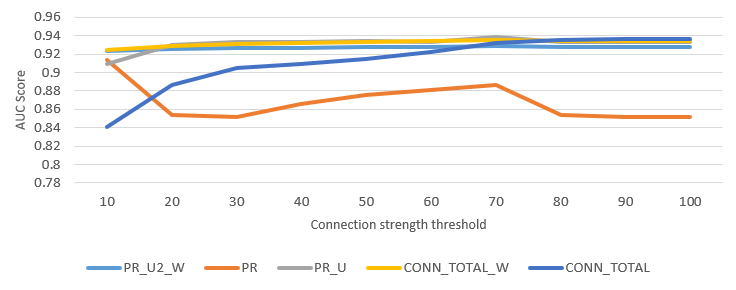
\includegraphics[width=\columnwidth]{ant_SD_LD.PNG}
\caption{Variation of AUC score when varying connection strength threshold for Ant. Results for structural and logical dependencies combined. }
\label{fig:plot_sd_ld_ant}
\centering
\end{figure}


\begin{figure}
\centering
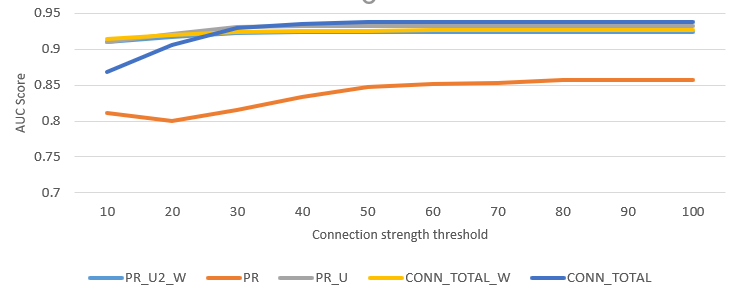
\includegraphics[width=\columnwidth]{tomcat_SD_LD.PNG}
\caption{Variation of AUC score when varying connection strength threshold for Tomcat. Results for structural and logical dependencies combined. }
\label{fig:plot_sd_ld_tomcat}
\centering
\end{figure}


\begin{figure}
\centering
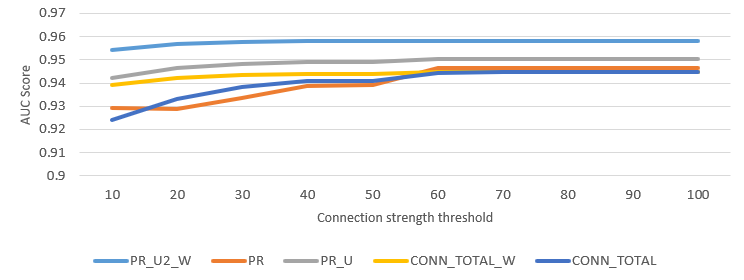
\includegraphics[width=\columnwidth]{hibernate_SD_LD.PNG}
\caption{Variation of AUC score when varying connection strength threshold for Hibernate. Results for structural and logical dependencies combined. }
\label{fig:plot_sd_ld_hibernate}
\centering
\end{figure}



\begin{figure}
\centering
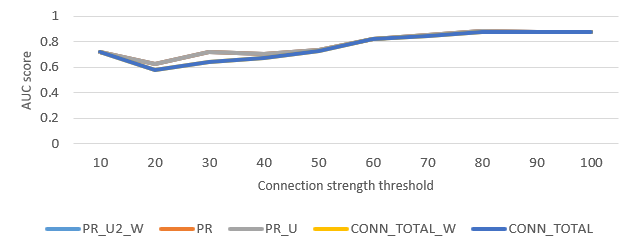
\includegraphics[width=\columnwidth]{ant_LD.PNG}
\caption{Variation of AUC score when varying connection strength threshold for Ant. Results for logical dependencies only. }
\label{fig:plot_ld_ant}
\centering
\end{figure}


\begin{figure}
\centering
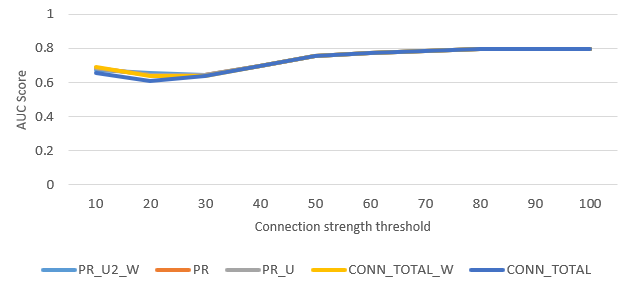
\includegraphics[width=\columnwidth]{tomcat_LD.PNG}
\caption{Variation of AUC score when varying connection strength threshold for Tomcat. Results for logical dependencies only. }
\label{fig:plot_ld_tomcat}
\centering
\end{figure}


\begin{figure}
\centering
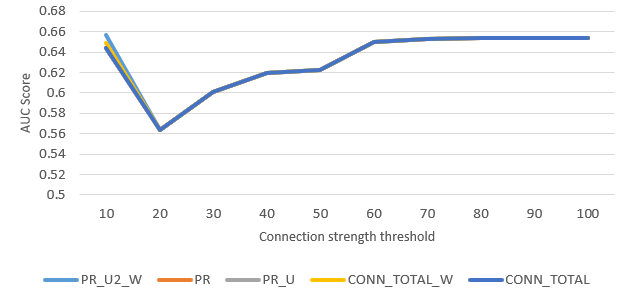
\includegraphics[width=\columnwidth]{hibernate_LD.PNG}
\caption{Variation of AUC score when varying connection strength threshold for Hibernate. Results for logical dependencies only.}
\label{fig:plot_ld_hibernate}
\centering
\end{figure}



Table \ref{tab:ratio_sd_ld} presents the ratio between the number of structural dependencies and logical dependencies. We included this table to highlight how different the total number of these two dependencies is.

\begin{table}[!h]
\renewcommand{\arraystretch}{1}
\caption{Percentage of logical dependencies that are also structural dependencies}
\label{tab:overlap}
\centering
\scalebox{0.7}{
\begin{tabular}{|c|cccccccccc|}
\hline
System &	$\geq10\%$	&	$\geq20\%$		&	$\geq30\%$		&	$\geq40\%$		&	$\geq50\%$		&	$\geq60\%$		&	$\geq70\%$		&	$\geq80\%$		&	$\geq90\%$		&	$\geq100\%$ \\
\hline
Ant	&	25.202	&	34.419	&	36.385	&	34.656	&	33.528	&	33.333	&	28.659	&	33.333	&	35.294	&	35.294	\\
Tomcat Catalina	&	4.059	&	22.089	&	25.000	&	25.758	&	25.926	&	37.525	&	47.368	&	55.285	&	75.000	&	76.923	\\
Hibernate	&	6.546	&	26.607	&	29.565	&	32.374	&	32.543	&	45.170	&	44.980	&	42.473	&	42.473	&	42.473	\\
\hline
\end{tabular}
}
\end{table}



\begin{table}[!h]
\renewcommand{\arraystretch}{1}
\caption{Ratio between structural and logical dependencies (SD/LD)}
\label{tab:ratio_sd_ld}
\centering
\scalebox{0.7}{
\begin{tabular}{|c|cccccccccc|}
\hline
System &	$\geq10\%$	&	$\geq20\%$		&	$\geq30\%$		&	$\geq40\%$		&	$\geq50\%$		&	$\geq60\%$		&	$\geq70\%$		&	$\geq80\%$		&	$\geq90\%$		&	$\geq100\%$ \\
\hline
Ant	&	1.315	&	3.284	&	4.972	&	5.603	&	6.175	&	10.697	&	12.915	&	27.154	&	41.529	&	41.529	\\
Tomcat Catalina	&	0.120	&	0.923	&	1.313	&	1.531	&	1.619	&	3.177	&	7.092	&	13.146	&	67.375	&	124.385	\\
Hibernate	&	1.037	&	6.391	&	10.037	&	14.947	&	18.940	&	54.248	&	83.442	&	111.704	&	111.704	&	111.704	\\

\hline
\end{tabular}
}
\end{table}

Figures \ref{fig:plot_sd_ld_ant}, \ref{fig:plot_sd_ld_tomcat}, and \ref{fig:plot_sd_ld_hibernate} show the measurements obtained by using structural and logical dependencies combined.

In all three figures, the initial measurements are lower than the rest. As the threshold value increases, the measurements also increase, indicating better results for key class detection. The best measurements are obtained when the threshold value is between 40 and 60. After this point, the measurements decrease slightly and stabilize at a fixed value. A possible explanation for this fluctuation and eventual stabilization is found in Table \ref{tab:ratio_sd_ld}. At the beginning, the total number of logical dependencies used is close to the number of existing structural dependencies. The high volume of logical dependencies introduced may cause incorrect key class detection, resulting in lower measurements.

As the threshold becomes more restrictive and the number of logical dependencies decreases, key class detection improves. This improvement stops after the threshold value reaches 60\%. Looking again at Table \ref{tab:ratio_sd_ld}, it can be observed that after 60\%, the number of structural dependencies outnumbers the number of logical dependencies by up to 124 times in some cases. Additionally, Table \ref{tab:overlap} shows that the remaining logical dependencies overlap significantly with the structural dependencies, meaning that not much new information is introduced at this point.
 So, the number of logical dependencies used is so small that it doesn't influence the key class identification. Since the structural dependencies used don't change, we obtain the same results for different threshold values \hspace{4em}. 



Figures \ref{fig:plot_ld_ant}, \ref{fig:plot_ld_tomcat}, and \ref{fig:plot_ld_hibernate} show the measurements obtained by using only logical dependencies. Initially, we expected to see a Gaussian curve, but instead, we observed a bell curve. This happens because, in the beginning, we use a high number of logical dependencies in key class detection. Among these logical dependencies, there is a significant number of key and non-key classes. However, non-key classes do not influence key class detection at this stage.

As we increase the threshold value and filter more logical dependencies, some of the initially detected key classes are filtered out. In this situation, the remaining non-key classes influence the measurements negatively, causing worse-performing results. Some key classes are strongly connected in the versioning system and remain even when higher threshold values are applied. At the same time, the non-key classes get filtered out at higher threshold values, leading to better-performing measurements when the threshold value exceeds 60\%.




\section{Comparison with fan-in and fan-out metric}
\label{sec:key_metrics}


\hspace{4em}Fan-in and fan-out are coupling metrics. The fan-in of entity A is the total number of entities that call functions of A, while the fan-out of A is the total number of entities that A calls functions from \cite{5507329}. Tables \ref{tab:measurementsfan:ant}, \ref{tab:measurementsfan:catalina}, and \ref{tab:measurementsfan:hibernate} present the detailed metrics for each documented key class in each system. 

The first column represents the name of each key class. The second column represents the fan\_in values for each key class, while the third column represents the fan\_out values. The fourth column represents the total number of entities interacting with the key class, calculated as the sum of fan\_in and fan\_out. The fifth column represents the number of logical dependencies (LD\_NUMBER) involved in each entity.

For Ant, Table \ref{tab:measurementsfan:ant} shows that all key classes have logical dependencies with other classes. The key classes with the highest number of logical dependencies are \texttt{Project} and \texttt{IntrospectionHelper}. These two entities also appear in Table \ref{tab:measurementstop:ant}, where we list the top 10 entities with logical dependencies. This indicates that some key classes are frequently involved in software changes, which can be observed through the system’s versioning history.


\begin{table}[!h]
\renewcommand{\arraystretch}{1}
\caption{Measurements for Ant key classes}
\label{tab:measurementsfan:ant}
\centering
\scalebox{0.8}{
\begin{tabular}{|c|ccccc|}
\hline
Nr.	&	Classname	&	FAN\_IN	&	FAN\_OUT	&	FAN\_TOTAL	&	LD\_NUMBER\\
\hline
1	&	Project	&	191	&	23	&	214	&	157	\\
2	&	Target	&	28	&	6	&	34	&	78	\\
3	&	UnknownElement	&	17	&	13	&	30	&	90	\\
4	&	RuntimeConfigurable	&	17	&	13	&	30	&	118	\\
5	&	IntrospectionHelper	&	18	&	24	&	42	&	143	\\
6	&	Main	&	1	&	13	&	14	&	82	\\
7	&	TaskContainer	&	11	&	1	&	12	&	21	\\
8	&	ProjectHelper2\$ElementHandler	&	1	&	12	&	13	&	30	\\
9	&	Task	&	110	&	7	&	117	&	88	\\
10	&	ProjectHelper	&	16	&	8	&	24	&	101	\\
\hline
\end{tabular}
}
\end{table}


For Tomcat Catalina, similar to Ant, Table \ref{tab:measurementsfan:catalina} shows that all key classes have logical dependencies. The key classes with the highest number of logical dependencies are \texttt{StandardContext} and \texttt{Request}. These two entities also appear in Table \ref{tab:measurementstop:catalina}, where we list the top 10 entities with the most logical dependencies in Tomcat Catalina.

For Hibernate, the situation is different. As seen in Table \ref{tab:measurementsfan:hibernate}, key classes like \texttt{Criterion}, \texttt{Projection}, and \texttt{Transaction} have zero logical dependencies, indicating that these key classes are not involved in any software change. One possible explanation for this is that Hibernate’s archi


\begin{table}[!h]
\renewcommand{\arraystretch}{1}
\caption{Measurements for Tomcat Catalina key classes.}
\label{tab:measurementsfan:catalina}
\centering
\scalebox{0.8}{
\begin{tabular}{|c|ccccc|}
\hline
Nr.	&	Classname	&	FAN\_IN	&	FAN\_OUT	&	FAN\_TOTAL	&	LD\_NUMBER \\
\hline
1	&	Context	&	74	&	8	&	82	&	126	\\
2	&	Request	&	48	&	28	&	76	&	215	\\
3	&	Container	&	51	&	8	&	59	&	64	\\
4	&	Response	&	38	&	12	&	50	&	90	\\
5	&	StandardContext	&	11	&	38	&	49	&	216	\\
6	&	FANector	&	23	&	9	&	32	&	89	\\
7	&	Session	&	29	&	2	&	31	&	28	\\
8	&	Valve	&	29	&	2	&	31	&	19	\\
9	&	Wrapper	&	29	&	1	&	30	&	36	\\
10	&	Manager	&	25	&	3	&	28	&	31	\\
11	&	Host	&	26	&	1	&	27	&	44	\\
12	&	Service	&	20	&	6	&	26	&	51	\\
13	&	Engine	&	23	&	2	&	25	&	1	\\
14	&	Realm	&	18	&	6	&	24	&	21	\\
15	&	CoyoteAdapter	&	1	&	22	&	23	&	140	\\
16	&	StandardHost	&	8	&	15	&	23	&	88	\\
17	&	LifecycleListener	&	21	&	1	&	22	&	3	\\
18	&    StandardEngine	&	2	&	19	&	21	&	57	\\
19	&	Pipeline	&	19	&	2	&	21	&	20	\\
20	&	Server	&	16	&	4	&	20	&	49	\\
21	&	HostConfig	&	3	&	15	&	18	&	79	\\
22	&	StandardWrapper	&	5	&	13	&	18	&	92	\\
23	&	StandardService	&	3	&	12	&	15	&	81	\\
24	&	Catalina	&	2	&	13	&	15	&	94	\\
25	&	Loader	&	14	&	1	&	15	&	18	\\
26	&	StandardServer	&	2	&	12	&	14	&	94	\\
27	&	StandardPipeline	&	1	&	10	&	11	&	62	\\
28	&	Bootstrap	&	3	&	3	&	6	&	41	\\	
\hline
\end{tabular}
}
\end{table}

\begin{table}[!h]
\renewcommand{\arraystretch}{1}
\caption{Measurements for Hibernate key classes.}
\label{tab:measurementsfan:hibernate}
\centering
\scalebox{0.8}{
\begin{tabular}{|c|ccccc|}
\hline
Nr.	&	Classname	&	FAN\_IN	&	FAN\_OUT	&	FAN\_TOTAL	&	LD\_NUMBER \\
\hline
1	&	SessionFactoryImplementor	&	438	&	43	&	481	&	51	\\
2	&	Type	&	444	&	5	&	449	&	0	\\
3	&	Table	&	89	&	29	&	118	&	82	\\
4	&	SessionImplementor	&	52	&	12	&	64	&	14	\\
5	&	Criteria	&	45	&	12	&	57	&	15	\\
6	&	Column	&	46	&	10	&	56	&	20	\\
7	&	Session	&	31	&	21	&	52	&	52	\\
8	&	Query	&	12	&	28	&	40	&	0	\\
9	&	Configuration	&	1	&	38	&	39	&	115	\\
10	&	SessionFactory	&	24	&	12	&	36	&	33	\\
11	&	Criterion	&	30	&	3	&	33	&	0	\\
12	&	Projection	&	11	&	3	&	14	&	0	\\
13	&	FANectionProvider	&	12	&	2	&	14	&	0	\\
14	&	Transaction	&	11	&	1	&	12	&	0	\\
				
\hline
\end{tabular}
}
\end{table}


%%%%%%%%%%%%%%%%%%%%%%%%%%%%%%%%%%%%%%%%%%%%%%%%%%%%%%%%%%%%%%%%%%%%%%%%%%%%%

Tables \ref{tab:measurementstop:ant}, \ref{tab:measurementstop:catalina}, and \ref{tab:measurementstop:hibernate} present the top 10 entities with the highest number of logical dependencies. The first column contains the names of the top 10 entities; the second column contains the fan\_in values, the third column contains the fan\_out values, the fourth column contains the combined fan\_in and fan\_out values, and the fifth column contains the number of logical dependencies (LD) involving each entity.

We created these top 10 tables to provide an overview of the highest LD numbers registered for each system. As mentioned, some key classes appear in these tables, but not all are included. In Table \ref{tab:measurementstop:hibernate}, which shows the top 10 entities for Hibernate, most entries are inner classes of \texttt{AbstractEntityPersister}. This is expected because the class \texttt{AbstractEntityPersister} is also listed. This behavior occurs due to the limitation of the versioning system, which cannot separate changes made to a class from those made to its inner classes. Therefore, whenever \texttt{AbstractEntityPersister} records a change, its inner classes are also marked as changed.

\begin{table}[!h]
\renewcommand{\arraystretch}{1}
\caption{Top 10 measurements for Ant. }
\label{tab:measurementstop:ant}
\centering
\scalebox{0.8}{
\begin{tabular}{|c|ccccc|}
\hline
Nr.	&	Classname	&	FAN\_IN	&	FAN\_OUT	&	FAN\_TOTAL	&	LD\_NUMBER \\
\hline
1	&	\cellcolor{lightorange}Project	&	191	&	23	&	214	&	157	\\
2	&	Project\$AntRefTable	&	1	&	2	&	3	&	157	\\
3	&	Path	&	39	&	13	&	52	&	147	\\
4	&	Path\$PathElement	&	3	&	2	&	5	&	147	\\
5	&	\cellcolor{lightorange}IntrospectionHelper	&	18	&	24	&	42	&	143	\\
6	&	IntrospectionHelper\$AttributeSetter	&	8	&	1	&	9	&	143	\\
7	&	IntrospectionHelper\$Creator	&	3	&	5	&	8	&	143	\\
8	&	IntrospectionHelper\$NestedCreator	&	7	&	1	&	8	&	143	\\
9	&	Ant	&	2	&	15	&	17	&	136	\\
10	&	Ant\$Reference	&	3	&	1	&	4	&	136	\\
\hline
\end{tabular}
}
\end{table}

\begin{table}[!h]
\renewcommand{\arraystretch}{1}
\caption{Top 10 measurements for Tomcat Catalina. }
\label{tab:measurementstop:catalina}
\centering
\scalebox{0.8}{
\begin{tabular}{|c|ccccc|}
\hline
Nr.	&	Classname	&	FAN\_IN	&	FAN\_OUT	&	FAN\_TOTAL	&	LD\_NUMBER \\
\hline
1	&	\cellcolor{lightorange}StandardContext	&	11	&	38	&	49	&	216	\\
2	&	StandardContext\$ContextFilterMaps	&	0	&	0	&	0	&	216	\\
3	&	StandardContext\$NoPluggabilityServletContext	&	0	&	0	&	0	&	216	\\
4	&	\cellcolor{lightorange}Request	&	48	&	28	&	76	&	215	\\
5	&	Request\$SpecialAttributeAdapter	&	0	&	0	&	0	&	215	\\
6	&	ApplicationContext	&	3	&	22	&	25	&	158	\\
7	&	ApplicationContext\$DispatchData	&	0	&	0	&	0	&	158	\\
8	&	ContextConfig	&	3	&	26	&	29	&	143	\\
9	&	ContextConfig\$DefaultWebXmlCacheEntry	&	0	&	0	&	0	&	143	\\
10	&	ContextConfig\$JavaClassCacheEntry	&	0	&	0	&	0	&	143	\\
\hline
\end{tabular}
}
\end{table}


\begin{table}[!h]
\renewcommand{\arraystretch}{1}
\caption{Top 10 measurements for Hibernate. }
\label{tab:measurementstop:hibernate}
\centering
\scalebox{0.8}{
\begin{tabular}{|c|ccccc|}
\hline
Nr.	&	Classname	&	FAN\_IN	&	FAN\_OUT	&	FAN\_TOTAL	&	LD\_NR \\
\hline
1	&	AvailableSettings	&	1	&	0	&	1	&	205	\\
2	&	AbstractEntityPersister	&	9	&	143	&	152	&	190	\\
3	&	AbstractEntityPersister\$CacheEntryHelper	&	0	&	0	&	0	&	190	\\
4	&	AbstractEntityPersister\$InclusionChecker	&	0	&	0	&	0	&	190	\\
5	&	AbstractEntityPersister\$NoopCacheEntryHelper	&	0	&	0	&	0	&	190	\\
6	&	AbstractEntityPersister\$ReferenceCacheEntryHelper	&	0	&	0	&	0	&	190	\\
7	&	AbstractEntityPersister\$StandardCacheEntryHelper	&	0	&	0	&	0	&	190	\\
8	&	AbstractEntityPersister\$StructuredCacheEntryHelper	&	0	&	0	&	0	&	190	\\
9	&	Dialect	&	265	&	104	&	369	&	176	\\
10	&	SessionFactoryImpl\$SessionBuilderImpl	&	1	&	25	&	26	&	167	\\
\hline
\end{tabular}
}
\end{table}

Overall, by comparing the values of \texttt{FAN\_IN}, \texttt{FAN\_OUT}, \texttt{FAN\_TOTAL}, and the number of logical dependencies in which a class is involved, we could not identify a direct connection between these metrics. Similarly, we cannot conclude that one metric directly influences the others. However, even though these metrics are not directly related, we believe that using them together can provide a more comprehensive view of the system’s connections and dependencies.



\section{Chapter conclusions}
\label{sec:key_class_conclusions}

\hspace{4em}This chapter studied the filtering and usage of co-changes extracted from the versioning system. We approached two scenarios for detecting key classes using logical dependencies. In the first scenario, we used logical and structural dependencies; in the second scenario, we used only logical ones. We adapted the tool used in the baseline approach for detecting key classes from structural dependencies \cite{Finding-key-classes} to process in addition also logical dependencies.

Even though the approaches differed, most related research used the ROC-AUC metric to evaluate the quality of results, as we did. Osman et al. achieved an average ROC-AUC score of 0.750 \cite{6676885}, Thung et al. obtained a score of 0.825 \cite{rocclasification}, and Şora et al. (our baseline approach) achieved an average score of 0.894 \cite{Finding-key-classes}.

In our research, we obtained an average ROC-AUC score of 0.916 when using logical and structural dependencies and a score of 0.791 when using only logical dependencies to detect key classes.

When using both types of dependencies combined, we achieved a slightly better ROC-AUC score than the one from the baseline approach. When using only logical dependencies, although we did not surpass the baseline score, our results were comparable to those obtained by other researchers. Based on these results, we observed a slight improvement in key class detection when using both logical and structural dependencies, with the best results achieved at a connection strength threshold between 40 and 70. Our connection strength metric also performed better than the confidence metric used in related research. When using only logical dependencies, the results were less effective than when using structural dependencies alone or when combining both types. However, the results were still comparable to those achieved by other researchers using only structural dependencies. We consider this a significant finding, as this research uses a different type of input: logical dependencies.

This opens the door to new research possibilities across various fields that rely on structural dependencies to gain insight into software systems. Since logical dependencies are easy and fast to extract from the versioning system and are not dependent on the programming language, their integration comes at a low cost.

In conclusion, logical dependencies can be used to gain valuable knowledge about software systems. Their main advantage is that they rely solely on data extracted from the versioning system and can be generalized to various programming languages.
